\documentclass{l4proj}
\usepackage{style}
\title{\emph{rmt}: Ross's Monitoring Tool}
\author{Ross Eric Barnie}
\begin{document}
\maketitle
\tableofcontents
\listoffigures
\renewcommand{\abstractname}{Acknowledgements}
\begin{abstract}
I would like to thank David White for his endless patience, advice and for always ending our meetings with the phrase, ``Go achieve!''.
Additionally I would like to thank the School of Computer Science in general who have for the vast majority of my time at University of Glasgow been extremely supportive.

\end{abstract}


\pagenumbering{arabic}
\chapter{Introduction}
``rmt'' or Ross's Monitoring Tool is a network monitoring tool 
designed to work with the University of Glasgow's Raspberry Pi 
Cloud. It's primary purpose is to provide an at-a-glance view of the 
status and resource usage of each Raspberry Pi and their respective 
Linux containers.

\section{Raspberry Pi Cloud}
\label{intro:picloud}

The University of Glasgow's Raspberry Pi Cloud \citep{glapicloud, picloudblog} (which will now be 
referred to as PiCloud, not to be confused with PiCloud Inc. \citeyearpar{picloudinc}) is not 
wholly unique, as other institutions have created similar projects.



\chapter{Context}
\section{University of Southampton Raspberry Pi Supercomputer}
\label{intro:pisupercomp}

It should be noted that University of Southampton also created a cluster of Raspberry Pi devices and before the University of Glasgow did according to the PiCloud blog \citep{picloudonsouthampton}, however theirs was designed to create a single, miniature super-computer.
This is sufficiently different in design and purpose from PiCloud as to disregard it for the purposes of this study.
\section{Docker}
\label{sec:docker}
Docker \citep{docker} is a container management tool that packages applications as lightweight containers.
It is already used within the PiCloud on the command line to manage its containers, however monitoring these is a long process based on terminal commands on individual hosts.
Considering the PiCloud has 56 hosts with the possibility of expansion, it would be unreasonable to expect these commands to continue to be done via individual terminal commands, hence the need for \emph{rmt}.
 
 \subsection{DockerUI}
 Docker has another project that provides a web interface which runs client-side so there is the possibility of a user-friendly way to monitor running (or not) containers.
 As can be seen in figure \ref{fig:dockerUiContainers}, the interface shows running containers and the applications those containers are running and the status of the container.
 This is useful information, however it monitors a single host, rather than multiple.

 \begin{figure}[t]
 	\centering
	\setlength\fboxsep{0pt}
	\setlength\fboxrule{0.5pt}
	\fbox{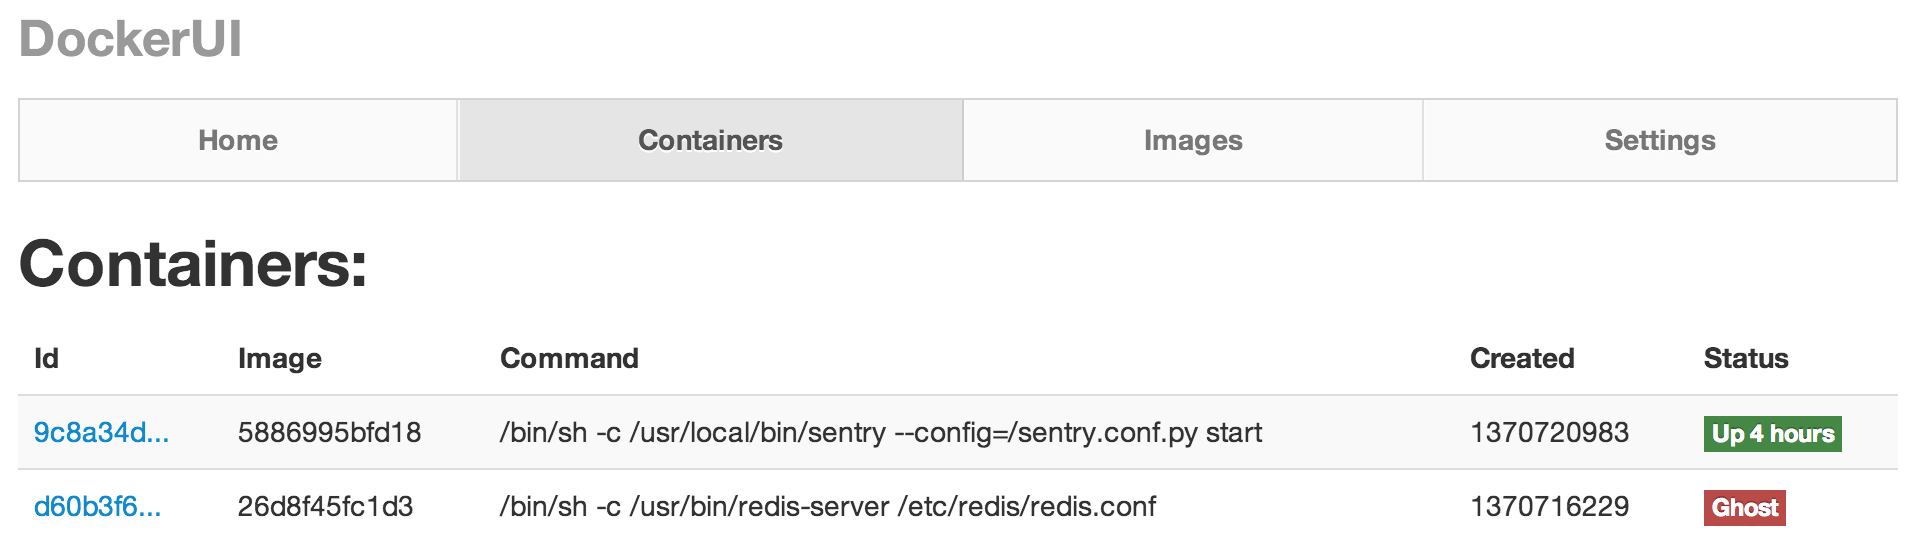
\includegraphics[width=0.8\textwidth]{dockerUiContainers}}
 	\caption{Containers overview in DockerUI}
 	\label{fig:dockerUiContainers}
 \end{figure}

 DockerUI's stated goals are more about wrapping docker functionality into a web app on a single client than acting as a cluster monitor, meaning it is unsuitable for use within \emph{rmt}.

\section{Shipyard}
Shipyard \citep{shipyard} is a web-based user interface for docker.
In many ways the functionality of shipyard meets the requirements of \emph{rmt}, outlined in section [reference], as it has the ability to monitor containers and multiple hosts.
However, the application has little ``at-a-glance'' features relevant to \emph{rmt}.
For example, to view all hosts in the application, the user has to enter a separate menu, shown in figure \ref{fig:shipyardHosts}.
This page displays only the network information about the host, such as hostname and port, and no system resource information.
Given the limited resources available on the Raspberry Pi boards, resource monitoring is a crucial component of any monitoring tool to be used with the PiCloud, so Shipyard would not be an appropriate option for use with the PiCloud.

Some design features were noted however, and these are outlined in section \ref{sec:implUi}.

\begin{figure}[t]
	\centering
	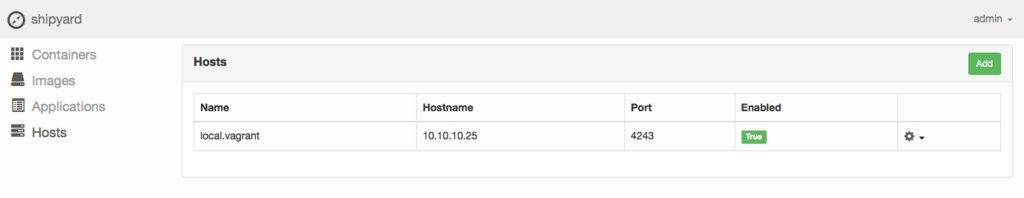
\includegraphics[width=0.8\textwidth]{shipyardHosts}
	\caption{Hosts page in Shipyard}
	\label{fig:shipyardHosts}
\end{figure}

% USE THIS SOMEWHERE ELSE (GUI implementation)
\begin{figure}[t]
	\centering
	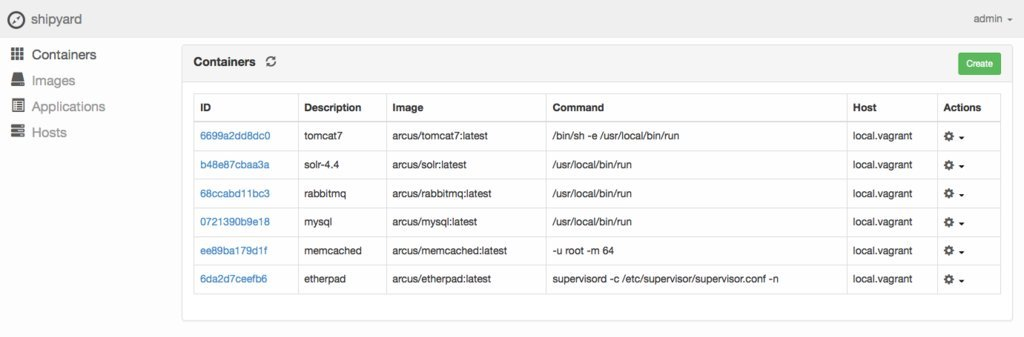
\includegraphics[width=0.8\textwidth]{shipyardContainers}
	\caption{Containers page in Shipyard}
	\label{fig:shipyardContainers}
\end{figure}

\chapter{Design}
\section{Methodology}
From the beginning of the project there was a need for rapid prototyping since many of the design decisions would be made during implementation.
To enable this, the design methodology chosen was that of ``Scrum''.

\subsection{Scrum Overview: Needs References}
Scrum is an agile software development methodology designed around the idea of work ``sprints''.
These consist of a unit of work, the design of which generally remains up to the ``Scrum Master'', who also oversees the proper use of the scrum methodology.
Each sprint is designed to add some feature to the implementation, whether it be an enhancement of previous features, or addition of entirely new features.
The length of time each sprint takes is variable, with some companies taking on daily scrum meetings to discuss sprints and others weekly.
This intuitively changes the amount of work expected to be done with each sprint.
There are three roles associated with scrums, one being the aforementioned ``Scrum Master'', the others being the ``Product Owner'' and the ``Development Team''.
The product owner represents the stakeholders, communicating their needs to the development team.
In this case the product owner was the supervisor of the project, David White, representing the other contributors to the PiCloud project, and also aided in managing sprints, thereby taking on some of the role of scrum master.
Intuitively, the development team was myself.
\section{Requirements Gathering}
Requirements were discussed in weekly meetings with the aforementioned product owner and supervisor of the project, David White.
These requirements were then noted and added to the Trello page for the project, further discussed in section \ref{sec:trello}, and given a priority of one of: ``Must have'', ``Should have'', ``Could have'', ``Would like to have'', commonly known as the MoSCoW framework.

\subsection{Must Have}
\label{sec:musthave}
\begin{description}
	\item[Keep client daemon(s) lightweight] given the Raspberry Pi's lack of resources, any applications running should use as little resources as possible
	\item[Monitor all hosts] the user should be able to monitor all 56 hosts
	\item[``at-a-glance'' monitoring] the user should not have to scroll to view all 56 hosts
	\item[Monitor resource usage of all hosts] the system should be able to display a given host's resource usage (RAM and CPU usage)
	\item[Temperature monitoring] the system should display the temperature of a given host
	\item[Delete a host] the user should be able to delete hosts from the system to stop monitoring it
	\item[Server state persists after reboot] the system should remain the same after a reboot of Pi Master
	\item[Heartbeat] the application should include some kind of heartbeat to indicate whether a host is turned on and responding
\end{description}

\subsection{Should Have}
\label{sec:shouldhave}
\begin{description}
	\item[Reboot a host] the user should be able to reboot a host from the system
	\item[View historical data] there should be some graphs to show the user historical data regarding resource usage and temperature
	\item[Monitor resource usage of containers] monitoring the resources used by the containers
\end{description}

\subsection{Could Have}
\label{sec:couldhave}
\begin{description}
	\item[Extensibility] the application should be extensible
	\item[Scalability] the application should scale well to allow for additional hosts
	\item[Secure login] the user should have to log in to view the application to allow for remote access and user privileges
\end{description}

\subsection{Would like to have}
\label{sec:wouldhave}
\begin{description}
	\item[Non-monitoring container operations] any function related to containers that are not monitoring, such as:
	\begin{itemize}
		\item kill containers
		\item restart containers
		\item start containers
		\item stop containers
	\end{itemize}
	\item[create container images remotely] containers need an image to be created from, this could be done remotely
	\item[``nice'' website] the website should be user-friendly 
\end{description}
\section{Tools}
Most of the decisions regarding tools were made during implementation.
However the following tools were made to aid the design process or were made prior to implementation.
Those made during implementation are outlined in section [section reference to implementation tools].

\subsection{Trello}
Trello \citep{trello} is an organisation tool developed by Fog Creek Software [reference].
While marketed as a tool to organise anything, it was created initially to organise teams in an office setting \citep{trellolaunch}.
However it is extremely useful as a project management tool, even for solo projects such as this.

Using Trello, several lists were created to represent different stages of development.
The lists used for the majority of the project were as follows, and an example of these lists in action can be seen in figure \ref{fig:trello}:
\begin{description}
	\item[Backlog] The list of features to be implemented
	\item[Currently Working On] The features currently in development (could be translated to ``current sprint'')
	\item[Stopped: Needs Discussion] The list of features stopped because a design decision needs to be made
	\item[Ready for acceptance] The list of features ready to be shown to and accepted by the stakeholders
\end{description}

\begin{figure}[t]
	\centering
	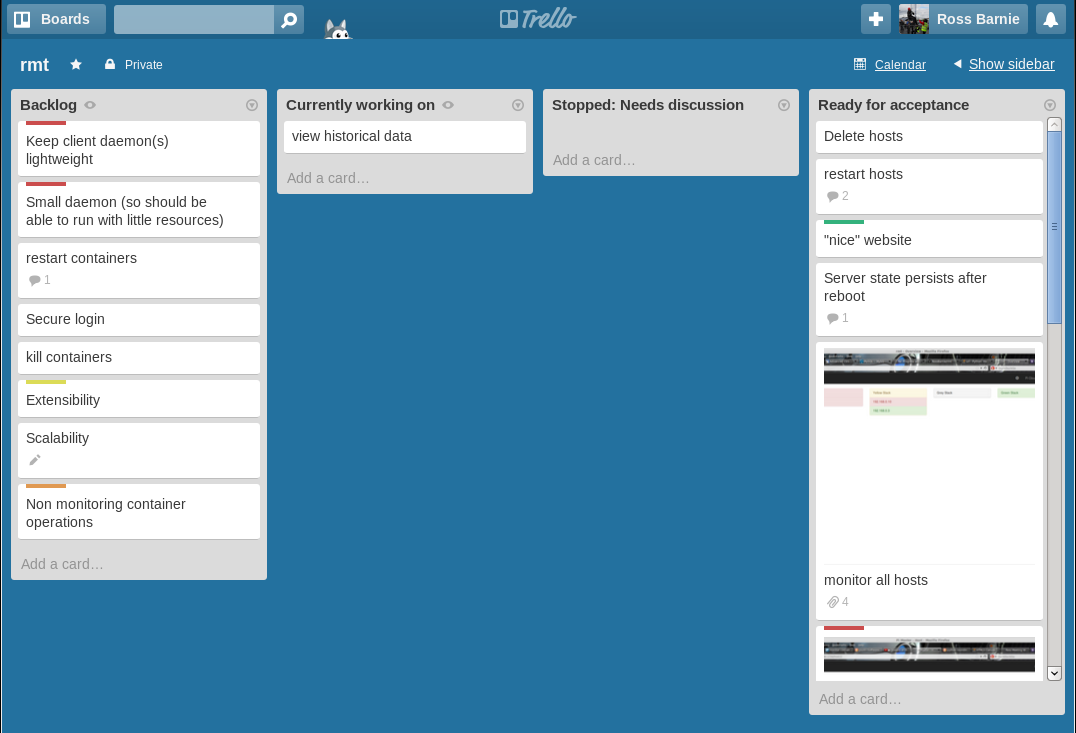
\includegraphics[width=0.8\textwidth]{rmtTrelloCurrent}
	\caption{Example usage of Trello during RMT development}
	\label{fig:trello}
\end{figure}

The Trello ``Board'' for the project was also made available to the project supervisor, David White.

As requirements were added, each was given a priority rating following the MoSCoW [reference] priority system and each was given a colour, as seen in figure \ref{fig:moscow}.

\begin{figure}[t]
	\centering
	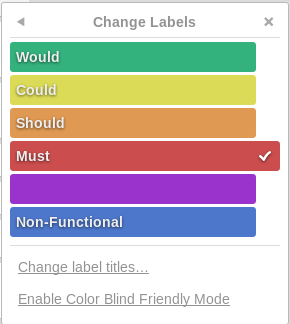
\includegraphics[width=0.3\textwidth]{moscowTrello}
	\caption{MoSCoW priorities as labels in Trello}
	\label{fig:moscow}
\end{figure}

\subsection{git and GitHub}
Version control is a key part of any software development project.
Having previous experience with and an account set up for GitHub \citeyearpar{github}, it was the obvious choice for this project, as well as this document in fact.

The project is currently set to private at \url{http://github.com/RossBarnie/rmt.git} to prevent public interaction however the repository will be made public (ie open-source) once it is no longer required to be developed by a single person.

\subsection{Python 2.7.6}
Python works very well in a rapid prototyping environment because it allows for applications to be coded quickly and easily, and the language itself is lightweight, catering to that requirement.
Not to mention its excellent documentation and number of different web frameworks available such as Django\citep{django}, webpy \citep{webpy} and web2py \citeyearpar{web2py}.

The legacy version (2.7.6) was chosen over newer versions (latest at time of writing is 3.4.0) because online resources for this version are exhaustive compared to newer versions and because of prior experience with it.
\section{Website Design}
\subsection{Initial Design}
During initial design meetings it was discussed that each host should have a graph representing the amount of resources (so, most likely CPU usage) each container is using on that host on the home page.

However, it became clear from early drafts of this design, which can be seen in figure \ref{fig:initialDesign}, that this would not display enough hosts without the need for the user to scroll which violates the ``at-a-glance'' requirement of the tool.

If the graphs were responsive, or calculating the values and updating the graphs in real time, it is expected that these graphs would require an unreasonable amount of load on the part of the client (the web browser accessing the website).
This is especially true if the number of hosts were to be as high as initially intended by the PiCloud project.

Additionally, there was no way of knowing, from a glance, which host belonged to which physical tower, which would be useful for diagnosis purposes, for example if a host was disconnected from its power supply. 

It is for these reasons that this design was abandoned.

\begin{figure}[t]
	\centering
	\setlength\fboxsep{0pt}
	\setlength\fboxrule{0.5pt}
	\fbox{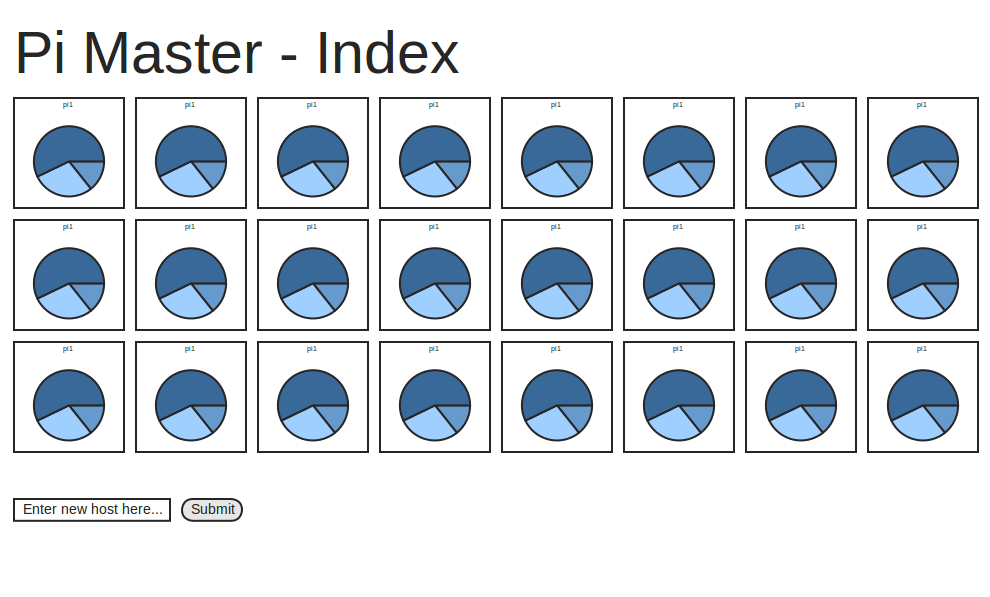
\includegraphics[width=0.8\textwidth]{rmtInitialDesign}}
	\caption{Initial design of \emph{rmt} home page}
	\label{fig:initialDesign}
\end{figure}

\subsection{Refined Design}

Following the lessons learned from the initial design, the home page would now simply list the hosts in such a way as to correspond to the tower they belonged to, and in text rather than graphs.
This would put far less load on the client (web browser accessing the page) and would be able to show more hosts without the need to scroll as much.
The design draft that followed can be seen in figure \ref{fig:refinedDesign}.

Both designs used the same amount of space (1000x600 pixels) yet immediately the user can see 60 hosts in the new design, compared to 24 in the previous design, and there is an immediate distinction between which host belongs to which tower.

\begin{figure}[t]
	\centering
	\setlength\fboxsep{0pt}
	\setlength\fboxrule{0.5pt}
	\fbox{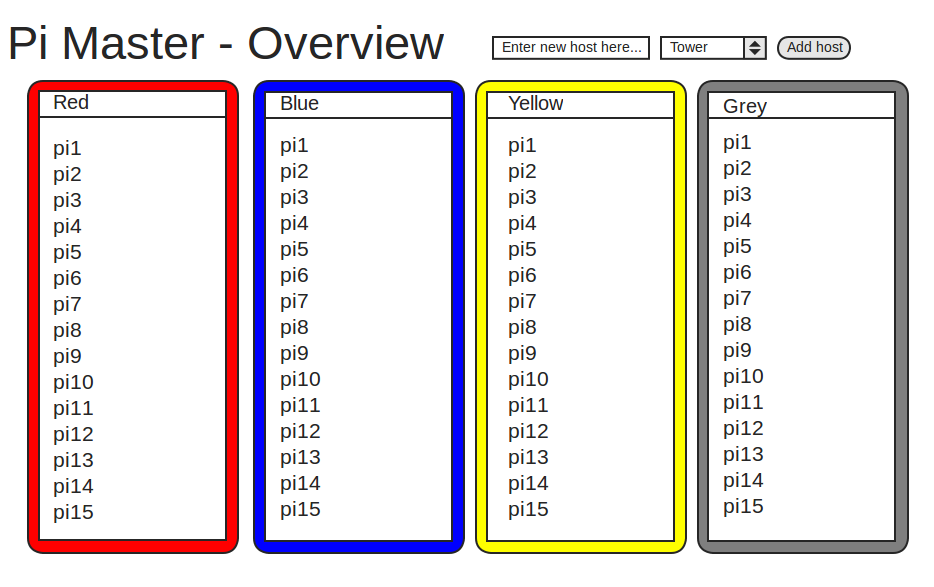
\includegraphics[width=0.8\textwidth]{rmtDesign}}
	\caption{Refined design of \emph{rmt} home page}
	\label{fig:refinedDesign}
\end{figure}

\chapter{Implementation}
\section{Architecture}
The architecture of \emph{rmt} is quite simple and a diagram showing the architecture can be seen in figure \ref{fig:arch} which will be referred to throughout this section.

\begin{figure}[t]
	\centering
	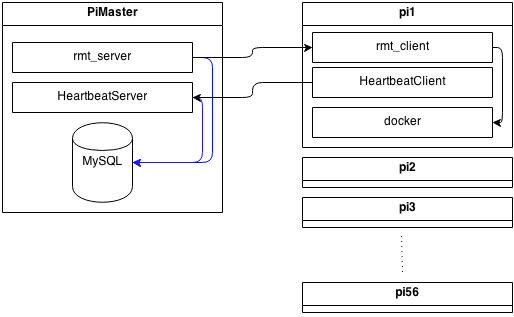
\includegraphics[width=0.6\textwidth]{rmtArch}
	\caption{diagram showing the architecture of \emph{rmt}}
	\label{fig:arch}
\end{figure}

\subsection{Overview}
The PiMaster has the \verb%rmt_server% application running which serves the web pages and retrieves data from the MySQL database and instances of \verb%rmt_client%.
PiMaster also has \verb%HeartbeatServer% running which listens on a specific port for messages from instances of \verb%HeartbeatClient%.

\verb%rmt_server% sends requests to \verb%rmt_client% via a REST interface for various pieces of information, the details of which are explained further in section [section reference].
Both \verb%rmt_server% and \verb%rmt_client% are web servers, the difference in names is to differentiate the server application from the application meant to be run on the hosts.

All of the Pi hosts have a software stack consisting of \verb%rmt_client%, \verb%HeartbeatClient%, and \verb%docker%.
There is no communication between \verb%rmt_client% and \verb%HeartbeatClient%.
\verb%rmt_client% and \verb%docker% communicate via a python wrapper module discussed in section \ref{impl:dockerpy}.

\subsection{rmt\_server}
POSSIBLY SWAP PLACES WITH CLIENT AS IT MAY MAKE MORE SENSE...

In accordance with the \verb%web.py% framework \citep{webpy}, each web page is assigned a class and that class deals with the logic behind the request either by using the class's \verb%GET% or \verb%POST% method, depending on the type of HTTP request.
The functions not defined as \verb%GET% or \verb%POST% are not exposed via a web interface and are simply regular python functions, following regular python scoping rules.

For example, the \verb%add% class in \verb%rmt_server.py% has three functions: \verb%GET%, \verb%POST%, and \verb%try_host%.
In this example, \verb%try_host% is inaccessible from the web, but is used within the \verb%POST% method to error check the host address being added by the user.

\subsection{rmt\_client}
The name of this module is somewhat misleading in that it is not a client at all.
It is actually a \verb%web.py% application and therefore a web server, exposing the following RESTful [need some references for REST] interface.

\begin{description}
	\item[GET /cpu] returns a json object corresponding to the cpu usage of the host in the same format as using \\\verb%psutil.cpu_times_percent%
	\item[GET /ram] returns a json object corresponding to the ram usage of the host in bits
	\item[GET /temperature] returns a json object containing a string with the temperature in [units]
	\item[GET /containers] returns a json object containing the equivalent output to \verb%docker ps% which lists all currently running containers
	\item[GET /reboot] returns a json object containing a message stating how many seconds it will be before a reboot takes place, and reboots the host
\end{description}

\subsection{HeartbeatServer and HeartbeatClient}

\subsection{MySQL Database}
Possibly include at least some of the creation script here.

\subsection{Docker}
The docker module seen in the architecture diagram is docker running on the client.
\section{Tools}
These differ from design tools in that these are tools not thought of during design but which were necessitated by something in the process of implementation.

\subsection{Dockerpy}
\label{impl:dockerpy}
Dockerpy \citep{dockerpy} is a python wrapper for docker functionality which was used in \emph{rmt} to interact with docker in the client application. 

\section{User Interface}
\label{sec:implUi}

\subsection{Home Page}
The User Interface (UI) for \emph{rmt}'s home page, seen in figure \ref{fig:rmtCurrent}, was based largely on the refined design seen in figure \ref{fig:refinedDesign}, so each host is assigned to a tower, represented by a Bootstrap panel, each with a different colour representing the colours of the physical towers seen in figure \ref{fig:pitowers}.
This parallel with the real world means that it is intuitive to understand which hosts belong to which tower.

There are minor differences between the finished product and the design in that the large header is removed in favour of a more conservative and Bootstrap-friendly header in the top left of the page.
This also provides the main link to the home page from any other page which many other websites employ (such as reddit \citep{reddit}, University of Glasgow's website \citep{glaWebsite}, and YouTube \citep{youtube}) in a similar fashion.

\subsubsection{Heartbeat State}
\label{sec:hbstate}
To aid the user in determining whether a host is running is achieved visually on the home page by the changing of colour of the host.
For example, the host with IP address 192.168.1.22 in figure \ref{fig:rmtCurrent} is grey, compared to the rest which are all green.
The green colour represents a ``fine'' state, meaning that the time in that host's \verb%last_contacted% field of the database table is within a configurable number of seconds, the default being three.
Once that number of seconds has been passed without contact, the state becomes the ``warning'' state, represented by a yellow colour, and once another configurable number of seconds has passed without contact (default is seven), the state changes to ``danger'' represented by a red colour.
And finally, the ``dead'' state, which is the state of 192.168.1.22 in figure \ref{fig:rmtCurrent}, triggers after another configurable number of seconds, the default being equivalent to a whole day (43200).

The configuration can be changed for this within the \verb%server.cfg% file, the related fields are shown below:

\begin{lstlisting}[caption={Configuration of heartbeat state times},label={lst:serverhbconfig}]
[heartbeat_visualisation]
danger_time = 7
warning_time = 3
dead_time = 43200
\end{lstlisting}

A state diagram showing this flow can be seen in figure \ref{fig:hbstate}.

\begin{figure}[t]
	\centering
	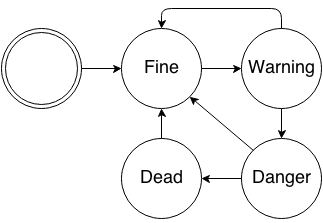
\includegraphics[scale=0.5]{state}
	\caption{State diagram of heartbeat state flow}
	\label{fig:hbstate}
\end{figure}

\subsection{Adding Hosts}

Adding hosts is no longer on the home page to make room for more hosts and because adding a host is not such a common operation that it needs to be on the home page.
In the case of PiCloud the add host form should be used to add the hosts to their corresponding towers and then left alone indefinitely until more Raspberry Pis are added to the PiCloud for example.
So instead of having the form on the home page, the form is on a separate page accessed by the plus icon in the top right of the home page (see figure \ref{fig:rmtCurrent}).

Next to this are links to the PiCloud website, since they were the ones to request the creation of this software, and a link to the GitHub page of \emph{rmt} since, as previously stated, the project will be made open source, and this provides an easy way for the user to find, and potentially contribute to, the project.

\begin{figure}[t]
	\centering
	\setlength\fboxsep{0pt}
	\setlength\fboxrule{0.5pt}
	\fbox{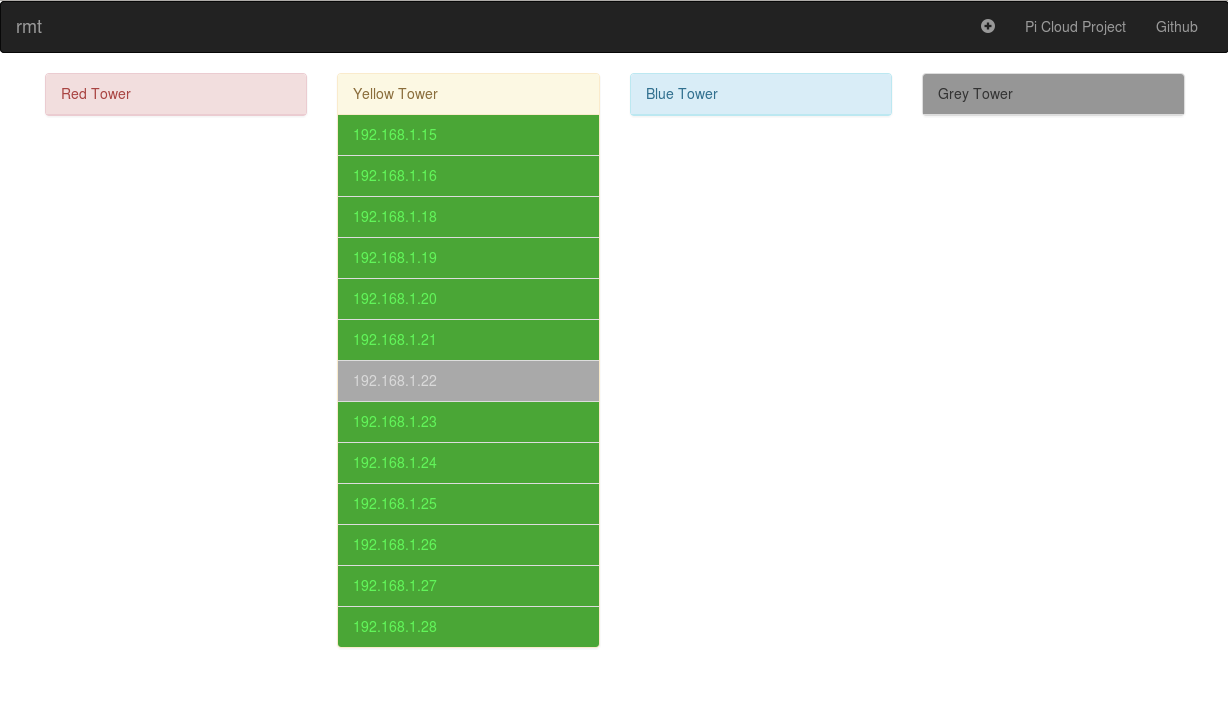
\includegraphics[width=0.8\textwidth]{rmtCurrent}}
	\caption{\emph{rmt}: home page}
	\label{fig:rmtCurrent}
\end{figure}

\begin{figure}[t]
	\centering
	\setlength\fboxsep{0pt}
	\setlength\fboxrule{0.5pt}
	\fbox{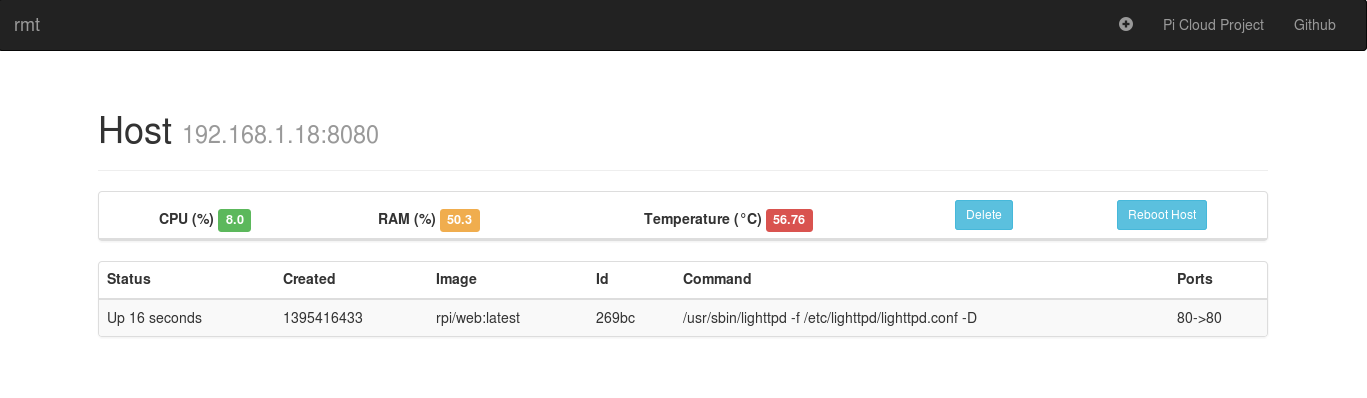
\includegraphics[width=0.8\textwidth]{rmtHostsCurrent}}
	\caption{\emph{rmt}: host page}
	\label{fig:rmtHostCurrent}
\end{figure}

\subsubsection{Host Page}

The design of the host page is somewhat inspired by the interface of Shipyard and DockerUI in that the table displayed shows similar fields.
Shipyard's container page (figure \ref{fig:shipyardContainers}) shows the Host field which \emph{rmt}'s host page does not need since this is already stated in the heading, and it shows the full ID of each container.
In \emph{rmt} the ID of the container is shortened to just five characters as this seemed sufficient to identify any containers running on a given host since, due to the Raspberry Pi's lack of resources, the number of containers actually able to run on any given Pi at once was so low as to be able to identify each container by the first five characters.
Additionally, the ``Description'' field seen in Shipyard's containers page was not available in the version of docker being used by PiCloud, so is not shown in \emph{rmt}'s host page.

The host page's container table actually more closely resembles DockerUI's containers table, shown in figure \ref{fig:dockerUiContainers}, though in a slightly different order and with fewer fields.
Admittedly the ``Status'' field in DockerUI is much more user-friendly with different labels to give more visual feedback to the user of the status of each container, however \emph{rmt} displays more fields, giving a better impression of what the containers are with the inclusion of the image name, and ports used in the case of running webservers.

\begin{figure}[t]
	\centering
	\setlength\fboxsep{0pt}
	\setlength\fboxrule{0.5pt}
	\fbox{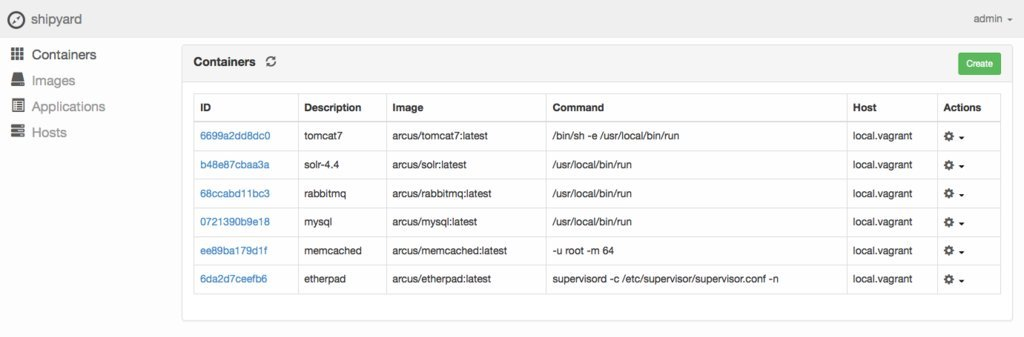
\includegraphics[width=0.8\textwidth]{shipyardContainers}}
	\caption{Containers page in Shipyard}
	\label{fig:shipyardContainers}
\end{figure}

By making the header, ``Host'', the user is reminded of where they are in the context of the system, and the sub-heading shows the user which host it is that they are viewing.
This includes the port of the client because there could feasibly be more than one client running on the same host.
This is entirely up to the systems administrator of the hosts but having more than one running instance of \verb%rmt_client% could add some redundancy to the host.

Labels throughout the system follow a colour scheme similar to that of the heartbeat states described earlier and are similarly configurable.

Buttons throughout the system are represented by Bootstrap's \verb%btn-info% class which is a light blue colour, making it visually distinctive to the status labels for CPU, RAM, and Temperature indicators, and the heartbeat states.



\chapter{Evaluation}


\chapter{Conclusion}
\section{Problems Encountered}
Throughout the development of \emph{rmt} many problems were encountered, some of which are outlined below.

\subsection{Google Charts}

Part of the reason the history graphs functionality was never completed was due to problems encountered when working with Google Charts \citeyearpar{googlecharts}.
Some of the problems were to do with lack of understanding of JavaScript \citep{javascript} and jQuery \citep{jquery}.

As explained in section \ref{sec:rmt_server}, web.py's templating language uses the dollar sign (\$) as a signal to begin a statement.
JQuery, which is automatically included in each of the pages used by \emph{rmt} since it is used by Bootstrap, also uses the dollar sign in its syntax.
With Google Charts using JavaScript, there was a conflict between web.py's templating language and jQuery.
This conflict was not picked up by web.py's debug mode, nor by Firefox's web development tools \citep{firefoxdevtools}, so no error message was displayed, but no graph was displayed.

After several failed attempts it was abandoned in favour of Flot \citep{flot}, which for reasons yet to reveal themselves, works even with the same dollar sign conflict problem as Google Charts.

\subsection{Web.py forms and Bootstrap form styling}

Using forms in web.py is relatively simple, as there are code samples on the web.py website explaining how to use them \citep{webpyform, webpyformfields}, however these do not include how to style individual fields, and neither does the API reference describing the web.py form class \citep{webpyformclass}.

After many failed attempts at constructing the form in the python codebase rather than in the template, it was decided to attempt to create the form in the HTML template, then manipulate the results in the python codebase.
This is now the form used in the add page.

\subsection{Development location}

Primarily the development of \emph{rmt} was completed at home and not at University of Glasgow's level 4 computing science laboratory for a number of reasons.

\begin{itemize}
	\item Root (administrator) access was required to run docker and allowing a student to have root access to the entire laboratory was out of the question, so programming the networking and docker-based functionality was far easier to do and test on a home network with full administrative privileges.
	\item Docker was not installed on the computers in the level 4 lab, though admittedly due to the previous point this was never requested.
	\item The disk space quota on the computers in the laboratory is limited and when trying to install modules it would fail due to lack of disk space, leading to wasted time trying to find items to delete.
\end{itemize}

Working from home was potentially not the only option available.
Requests could have been made for root access to a small subnet of computers or perhaps a remote authentication to the PiCloud itself could have been arranged, however this was never requested.

While it was the most convenient option it had a detrimental effect on ability to focus, as separating home life from university life proved problematic.
More of this project could have been completed had development occurred in an environment more conducive to learning and productivity, and though it is accepted that this was not the only problem related to productivity, it was certainly the largest contributing factor.
\section{Current State}
Currently \emph{rmt} meets all of the ``Must Have'' requirements outlined in section \ref{sec:musthave}.
Using python as the language may not be the fastest choice but it is lightweight, using little resources to run the client application thanks to the web.py framework.

The user can view all of the hosts on a single page depending on their screen resolution.
Development of \emph{rmt} was performed on a monitor with a 4:3 ratio and resolution of 1280x1024 and this was sufficient to display 56 hosts at a time.
Having a screen height of less than 800 pixels may require some scrolling, though modern monitors rarely have less than this, particularly in 4:3 ratio monitors.

``At-a-glance'' monitoring is accomplished through the heartbeat states, though is limited to showing simply whether a host is responding and any other information requires further navigation by the user.

Resource usage and temperature monitoring is similarly affected in that it requires navigation to a host to view.

Deleting and rebooting hosts is performed via buttons on the host page.

Server state is persistent thank to use of the database for heartbeats and because other host-relevant information is gathered by request of the host page and not stored locally.

The heartbeat requirement is fulfilled thanks to the heartbeat server and client discussed in section \ref{sec:heartbeat}.

As the evaluation discussed in section [reference] %\ref{sec:evaluation}
shows, the website is user-friendly and can therefore qualify as being a ``nice website''.

With the MySQL database being the key storage of the system, it should be scalable at least to the 1000 hosts initially intended by the PiCloud project however this is untested.

Extensibility is achieved in the sense that the code is readable, given the web.py framework's simple method of adding web-accessible methods, easy to follow.
If someone were to want to extend the project by adding a page for example, they would simply have to add a URL mapping, a class to handle the URL, a GET method within this, and then design the content of the page with a HTML file in the templates folder.


\section{Future Work}
\label{sec:future}
In the near future the code will be made open source.
While this is not expected to generate great interest in the open source community, given the almost bespoke nature of the software, it is of great personal interest to do so and some of the code that was not used but which exists for posterity will be removed to clean up the repository.

Historical graphs were in development and close to completion, so this will be the first feature to be implemented (currently this code resides in the history-graphs branch of the repository).
The history graphs are calculated using a new module which will be run periodically to gather the CPU, RAM, and temperature information from each host and add this to a new table in the database, as shown in figure \ref{fig:newArch}.

\begin{figure}[t]
	\centering
	\setlength\fboxsep{0pt}
	\setlength\fboxrule{0pt}
	\fbox{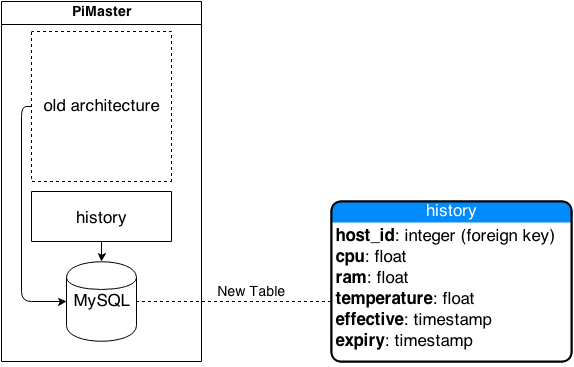
\includegraphics[scale=0.4]{newArch}}
	\caption{Proposed new architecture to allow for history graphs}
	\label{fig:newArch}
\end{figure}

Other functionality in the requirements but not fulfilled at this time are the priority of future work, as well as the changes recommended as a result of the evaluation, outlined in chapter \ref{sec:evaluation}.

The database does not necessarily have to be a MySQL database, and if someone were to want to use, for example, PostgreSQL instead, then this switch should be made easier by making it part of the configuration files.
It may require a different database creation script than the one currently in use but it should be a simple matter of parameterising the database object creation line in the database layer, and using the creation script related to the database the user wants.

\bibliography{ref}

\end{document}
